% THIS TEMPLATE IS A WORK IN PROGRESS
% Adapted from an original template by faculty at Reykjavik University, Iceland

\documentclass{scrartcl}
\input{File_Setup.tex}
\usepackage{graphicx,epsfig}
\hypersetup{
   colorlinks   = true,                               %Colours links instead of ugly boxes
   urlcolor     = blue,                               %Colour for external hyper links
   linkcolor    = blue,                               %Colour of internal links
   citecolor    = red,                                %Colour of citations
   setpagesize  = false,
   linktocpage  = true,
}
\graphicspath{ {fig/} }



\renewenvironment{abstract}{
    \centering
    \textbf{Abstract}
    \vspace{0.5cm}
    \par\itshape
    \begin{minipage}{0.7\linewidth}}{\end{minipage}
    \noindent\ignorespaces
}
% ------------------------------------------------------------------------------------------------------------------------

\begin{document}
%Title of the report, name of coworkers and dates (of experiment and of report).
\begin{titlepage}
	\centering
	\includegraphics[width=0.6\textwidth]{GW_logo.eps}\par
	\vspace{2cm}
	%%%% COMMENT OUT irrelevant lines below: Data Science OR Computer Science OR none
	{\scshape\LARGE Data Science Program \par}
	\vspace{1cm}
	{\scshape\Large Capstone Report - Fall 2024\par}
	%{\large \today\par}
	\vspace{1.5cm}
	%%%% PROJECT TITLE
	{\huge\bfseries MyRag - Advancing Retrieval-Augmented Generation and Comparative Analysis of Basic RAG, ColBERT Reranking, and RAPTOR Architecture\par}
	\vspace{2cm}
	%%%% AUTHOR(S)
	{\Large\itshape Meet Daxini \\}\par
	\vspace{1.5cm}
	supervised by\par
	%%%% SUPERVISOR(S)
	Amir Jafari
\newpage

	\vfill
	\begin{abstract}
Retrieval-Augmented Generation (RAG) systems are becoming increasingly popular for providing personalized, relevant, and current information in response to user queries by leveraging large language models (LLMs) and augmenting them with retrieved context. This paper presents MyRAG, an open-source RAG system that compares different models and architectures on two datasets. The system supports various embedding models, vector databases, LLMs, and advanced retrieval techniques like ColBERT re-ranking and the RAPTOR architecture. Evaluations on the BioASQ and Hugging Face Question Answering datasets demonstrate the effectiveness of different configurations. MyRAG aims to provide a versatile solution for efficient information retrieval and generation.
	\end{abstract}
	\vfill
% Bottom of the page
\end{titlepage}
\tableofcontents
\newpage
% ------------------------------------------------------------------------------------------------------------------------
\section{Introduction}

The exponential growth of digital data has made it challenging to efficiently retrieve relevant information to meet the increasing demand for personalized and up-to-date responses from LLMs. RAG systems address this by augmenting LLMs with retrieved context, enabling them to provide more accurate and current answers without hallucinations. With the expanding context window sizes of LLMs, RAG systems can leverage a large amount of relevant information to generate high-quality responses. This paper introduces MyRAG, an open-source RAG system that compares various models and architectures on different datasets, catering to both high-resource and resource-constrained environments.

% ------------------------------------------------------------------------------------------------------------------------
\section{Problem Statement}

Although there are numerous models and architectures for RAG, a comprehensive comparison of their performance on diverse datasets is needed. MyRAG aims to address this by implementing and evaluating popular and state-of-the-art approaches, including different embedding models, vector databases, LLMs, and advanced retrieval techniques like ColBERT reranking and the RAPTOR architecture. The system is designed to work with both high-compute resources and limited computational resources, making it suitable for various use cases. 

% ------------------------------------------------------------------------------------------------------------------------


\section{Related Work}

MyRAG builds upon existing work in the field of RAG systems, incorporating various components and techniques:

Embedding Models: The system supports several embedding models, such as NV-Embed-v2, Stella 1.5B, MXBai Large, Amazon Titan, and all-MiniLM-L6-v2, each with different model sizes and parameters.
Vector Databases: MyRAG utilizes Chroma and DeepLake for efficient vector storage and retrieval, leveraging techniques like Hierarchical Navigable Small World (HNSW) graphs and distance metrics such as cosine similarity and L2 distance.
LLMs: The system integrates various LLMs, including Llama 2, Mixtral, Gemma, and Hugging Face models, with different model sizes and parameters.
ColBERT Re-ranking: MyRAG incorporates the ColBERT model for fast and effective re-ranking of retrieved documents, as described in the ColBERT paper.
RAPTOR Architecture: The system implements the RAPTOR (Recursive Abstractive Processing for Tree-Organized Retrieval) architecture, adapting the code from the original paper to work with the MyRAG pipeline and databases.




% ------------------------------------------------------------------------------------------------------------------------

\section{MyRag}



\begin{figure}[H]
	\begin{center}
		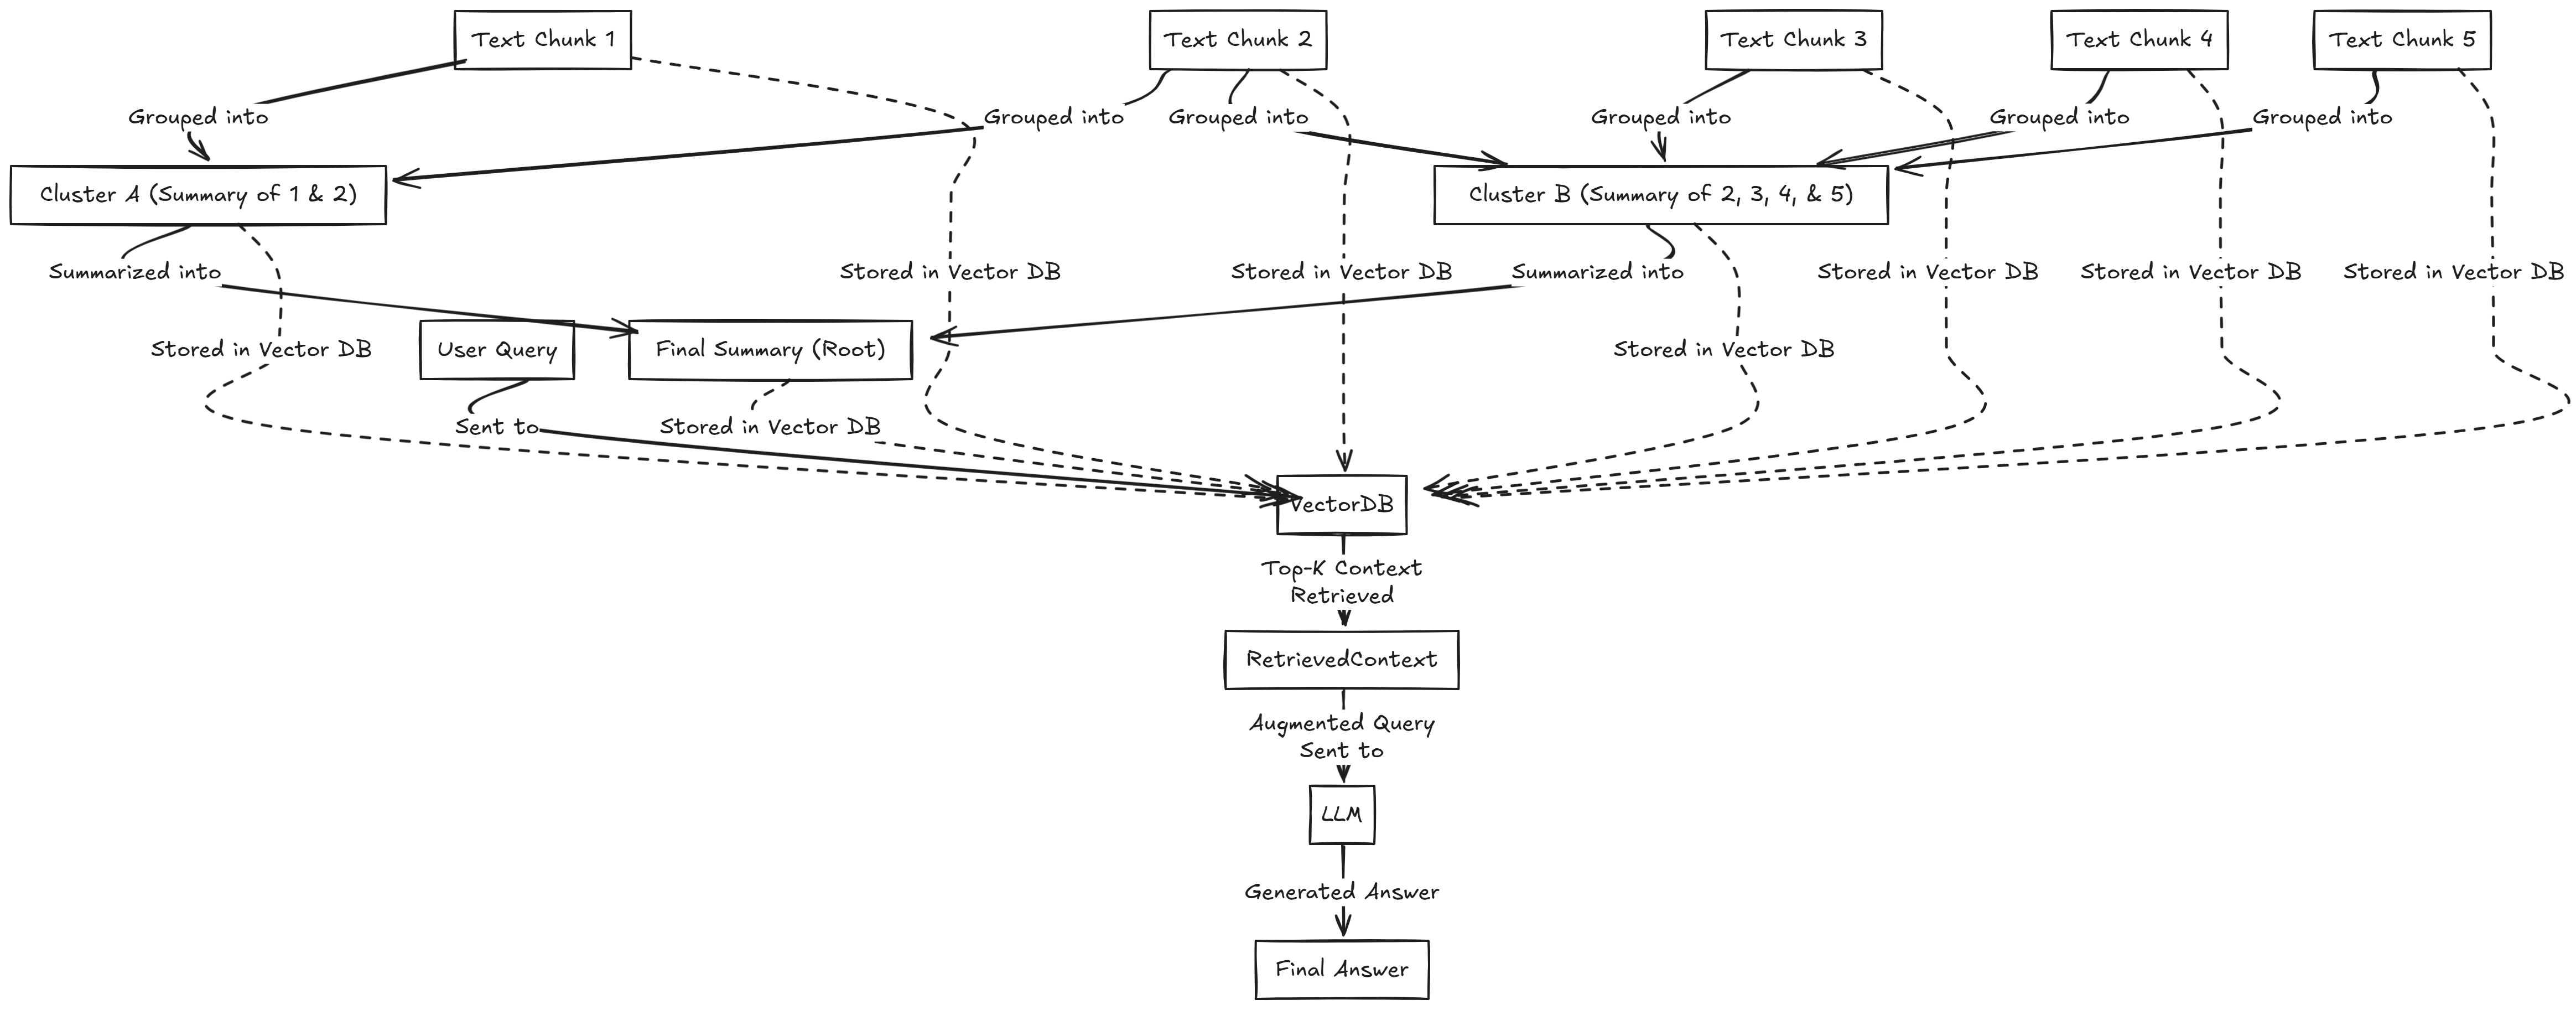
\includegraphics[scale=0.1]{raptor_final.png}
	\end{center}
	\caption{Raptor}
	\label{fig:ascent}
\end{figure}


% ------------------------------------------------------------------------------------------------------------------------
\section{Evaluations and Results}


\subsection{Result tables}

\begin{table}[H]
    \centering
    \caption{Retrieval Accuracies at Different k Values (With/Without Reranking)}
    \tiny
    \begin{tabular}{ll|cc|cc|cc|cc|cc}
    \hline
    \multirow{2}{*}{Model} & \multirow{2}{*}{Dataset} & \multicolumn{2}{c|}{k=1} & \multicolumn{2}{c|}{k=3} & \multicolumn{2}{c|}{k=5} & \multicolumn{2}{c|}{k=7} & \multicolumn{2}{c}{k=10} \\
    \cline{3-12}
    & & Base & +RR & Base & +RR & Base & +RR & Base & +RR & Base & +RR \\
    \hline
    NV-Embed-v2 & HuggingFace & .91 & .97 & .98 & .98 & .98 & .98 & 1.0 & .98 & 1.0 & 1.0 \\
    & PubMed & 1.0 & 1.0 & .79 & .74 & .77 & .78 & .79 & .80 & .80 & .82 \\
    \hline
    Stella 1.5B & HuggingFace & .95 & .95 & .98 & .98 & 1.0 & .98 & 1.0 & .98 & 1.0 & 1.0 \\
    & PubMed & 1.0 & 1.0 & .72 & .72 & .72 & .73 & .74 & .79 & .79 & .79 \\
    \hline
    MXBai Large & HuggingFace & .95 & .92 & .95 & .97 & .95 & .98 & .98 & .98 & .98 & .98 \\
    & PubMed & 1.0 & 1.0 & .77 & .77 & .74 & .74 & .77 & .80 & .79 & .82 \\
    \hline
    Titan Embed & HuggingFace & .89 & .92 & .95 & .95 & .98 & .95 & .98 & .95 & .98 & .98 \\
    & PubMed & 1.0 & 1.0 & .69 & .74 & .69 & .73 & .67 & .75 & .73 & .79 \\
    \hline
    MiniLM-L6 & HuggingFace & .58 & .88 & .72 & .89 & .77 & .91 & .80 & .91 & .83 & .91 \\
    & PubMed & .62 & .85 & .51 & .72 & .57 & .69 & .54 & .72 & .61 & .73 \\
    \hline
    \end{tabular}
    \label{tab:retrieval_accuracies}
\end{table}

\begin{table}[H]
    \centering
    \caption{Comprehensive Performance Comparison Across Models and Datasets basic rag and with reranking model}
    \small
    \begin{tabular}{llccccc}
    \hline
    Embedding Model & Dataset & Reranking & Total & Correct & Incorrect & Partial \\
    \hline
    \multirow{2}{*}{Titan Embed} & HuggingFace QA & None & 65 & 63 & 2 & 0 \\
    & PubMed & None & 13 & 8 & 0 & 5 \\
    \cline{2-7}
    & HuggingFace QA & ColBERT & 65 & 62 & 3 & 0 \\
    & PubMed & ColBERT & 13 & 8 & 0 & 5 \\
    \hline
    \multirow{2}{*}{Stella 1.5B} & HuggingFace QA & None & 65 & 64 & 1 & 0 \\
    & PubMed & None & 13 & 9 & 0 & 4 \\
    \cline{2-7}
    & HuggingFace QA & ColBERT & 65 & 63 & 2 & 0 \\
    & PubMed & ColBERT & 13 & 8 & 0 & 5 \\
    \hline
    \multirow{2}{*}{MXBai Large} & HuggingFace QA & None & 65 & 62 & 3 & 0 \\
    & PubMed & None & 13 & 8 & 1 & 4 \\
    \cline{2-7}
    & HuggingFace QA & ColBERT & 65 & 63 & 2 & 0 \\
    & PubMed & ColBERT & 13 & 8 & 0 & 5 \\
    \hline
    \multirow{2}{*}{NV-Embed-v2} & HuggingFace QA & None & 65 & 64 & 1 & 0 \\
    & PubMed & None & 13 & 9 & 1 & 3 \\
    \cline{2-7}
    & HuggingFace QA & ColBERT & 65 & 63 & 2 & 0 \\
    & PubMed & ColBERT & 13 & 8 & 0 & 5 \\
    \hline
    \multirow{2}{*}{MiniLM-L6} & HuggingFace QA & None & 65 & 50 & 15 & 0 \\
    & PubMed & None & 13 & 6 & 3 & 4 \\
    \cline{2-7}
    & HuggingFace QA & ColBERT & 65 & 58 & 7 & 0 \\
    & PubMed & ColBERT & 13 & 5 & 3 & 5 \\
    \hline
    \end{tabular}
    \label{tab:comprehensive_results}
\end{table}



\begin{table}[H]
    \centering
    \caption{Performance Comparison of Different Model Combinations Using Raptor Architecture}
    \begin{tabular}{llccc}
    \hline
    Embedding Model & Dataset & Total Questions & Correct & Partially Correct \\
    \hline
    Stella 1.5B & HuggingFace QA & 65 & 65 & 0 \\
    Stella 1.5B & PubMed & 13 & 10 & 3 \\
    MXBai Large & HuggingFace QA & 65 & 64 & 0 \\
    MXBai Large & PubMed & 13 & 9 & 3 \\
    \hline
    \end{tabular}
    \label{tab:model_performance}
\end{table}

\begin{table}[H]
\centering
\small
\begin{adjustbox}{max width=\textwidth}
\begin{tabular}{llp{5cm}cccccccccccccccccc}
\toprule
\textbf{Model} & \textbf{Dataset} & \textbf{Settings} & \textbf{Accuracy@1} & \textbf{Accuracy@1 After Rerank} & \textbf{Accuracy@2} & \textbf{Accuracy@2 After Rerank} & \textbf{Accuracy@3} & \textbf{Accuracy@3 After Rerank} & \textbf{Accuracy@4} & \textbf{Accuracy@4 After Rerank} & \textbf{Accuracy@5} & \textbf{Accuracy@5 After Rerank} & \textbf{Accuracy@6} & \textbf{Accuracy@6 After Rerank} & \textbf{Accuracy@7} & \textbf{Accuracy@7 After Rerank} & \textbf{Accuracy@8} & \textbf{Accuracy@8 After Rerank} & \textbf{Accuracy@9} & \textbf{Accuracy@9 After Rerank} & \textbf{Accuracy@10} & \textbf{Accuracy@10 After Rerank} \\
\midrule
\texttt{nvidia/NV-Embed-v2} & \texttt{HuggingFace QA Dataset} & \texttt{\{'name': 'nvidia/NV-Embed-v2', 'batch\_size': 2, 'query\_instruction': 'Instruct: Given a question, retrieve passages that answer the question.\textbackslash nQuery:', 'model\_kwargs': \{'trust\_remote\_code': True, 'load\_in\_8bit': True, 'max\_length': 32768\}\}} & 0.91 & 0.97 & 0.94 & 0.98 & 0.98 & 0.98 & 0.98 & 0.98 & 0.98 & 0.98 & 0.98 & 0.98 & 1.0 & 0.98 & 1.0 & 1.0 & 1.0 & 1.0 & 1.0 & 1.0 \\
\texttt{dunzhang/stella\_en\_1.5B\_v5} & \texttt{HuggingFace QA Dataset} & \texttt{\{'name': 'dunzhang/stella\_en\_1.5B\_v5', 'batch\_size': 2, 'query\_instruction': 'Instruct: Given a web search query, retrieve relevant passages that answer the query.\textbackslash nQuery:', 'model\_kwargs': \{'trust\_remote\_code': True\}\}} & 0.95 & 0.95 & 0.98 & 0.98 & 0.98 & 0.98 & 0.98 & 0.98 & 1.0 & 0.98 & 1.0 & 0.98 & 1.0 & 0.98 & 1.0 & 0.98 & 1.0 & 1.0 & 1.0 & 1.0 \\
\texttt{dunzhang/stella\_en\_1.5B\_v5} & \texttt{HuggingFace QA Dataset} & \texttt{\{'name': 'dunzhang/stella\_en\_1.5B\_v5', 'batch\_size': 2, 'query\_instruction': 'Instruct: Given a web search query, retrieve relevant passages that answer the query.\textbackslash nQuery:', 'model\_kwargs': \{'trust\_remote\_code': True, 'load\_in\_8bit': True\}\}} & 0.88 & 0.77 & 0.91 & 0.77 & 0.91 & 0.77 & 0.91 & 0.77 & 0.92 & 0.78 & 0.94 & 0.78 & 0.94 & 0.78 & 0.94 & 0.78 & 0.94 & 0.82 & 0.94 & 0.82 \\
\texttt{sentence-transformers/all-MiniLM-L6-v2} & \texttt{HuggingFace QA Dataset} & \texttt{\{'name': 'sentence-transformers/all-MiniLM-L6-v2', 'batch\_size': 100\}} & 0.58 & 0.88 & 0.66 & 0.89 & 0.72 & 0.89 & 0.74 & 0.89 & 0.77 & 0.91 & 0.80 & 0.91 & 0.80 & 0.91 & 0.82 & 0.91 & 0.83 & 0.91 & 0.83 & 0.91 \\
\texttt{mixedbread-ai/mxbai-embed-large-v1} & \texttt{HuggingFace QA Dataset} & \texttt{\{'name': 'mixedbread-ai/mxbai-embed-large-v1', 'batch\_size': 100\}} & 0.95 & 0.92 & 0.95 & 0.97 & 0.95 & 0.97 & 0.95 & 0.98 & 0.95 & 0.98 & 0.97 & 0.98 & 0.98 & 0.98 & 0.98 & 0.98 & 0.98 & 0.98 & 0.98 & 0.98 \\
\texttt{amazon.titan-embed-text-v2:0} & \texttt{HuggingFace QA Dataset} & \texttt{\{'name': 'amazon.titan-embed-text-v2:0', 'model\_kwargs': \{'aws': True, 'aws\_creds\_file': '/home/ubuntu/Multi-Agent-LLM-System-with-LangGraph-RAG-and-LangChain/config/config.ini', 'aws\_config\_name': 'BedRock\_LLM\_API'\}\}} & 0.89 & 0.92 & 0.91 & 0.95 & 0.95 & 0.95 & 0.97 & 0.95 & 0.98 & 0.95 & 0.98 & 0.95 & 0.98 & 0.95 & 0.98 & 0.97 & 0.98 & 0.98 & 0.98 & 0.98 \\
\texttt{nvidia/NV-Embed-v2} & \texttt{PubMed filtered Dataset} & \texttt{\{'name': 'nvidia/NV-Embed-v2', 'batch\_size': 2, 'query\_instruction': 'Instruct: Given a question, retrieve passages that answer the question.\textbackslash nQuery:', 'model\_kwargs': \{'trust\_remote\_code': True, 'load\_in\_8bit': True, 'max\_length': 32768\}\}} & 1.0 & 1.0 & 0.85 & 0.81 & 0.79 & 0.74 & 0.76 & 0.77 & 0.77 & 0.78 & 0.76 & 0.81 & 0.79 & 0.80 & 0.80 & 0.80 & 0.80 & 0.80 & 0.80 & 0.82 \\
\texttt{dunzhang/stella\_en\_1.5B\_v5} & \texttt{PubMed filtered Dataset} & \texttt{\{'name': 'dunzhang/stella\_en\_1.5B\_v5', 'batch\_size': 2, 'query\_instruction': 'Instruct: Given a web search query, retrieve relevant passages that answer the query.\textbackslash nQuery:', 'model\_kwargs': \{'trust\_remote\_code': True\}\}} & 1.0 & 1.0 & 0.73 & 0.85 & 0.72 & 0.72 & 0.71 & 0.67 & 0.72 & 0.73 & 0.72 & 0.77 & 0.74 & 0.79 & 0.75 & 0.79 & 0.76 & 0.79 & 0.79 & 0.79 \\
\texttt{dunzhang/stella\_en\_1.5B\_v5} & \texttt{PubMed filtered Dataset} & \texttt{\{'name': 'dunzhang/stella\_en\_1.5B\_v5', 'batch\_size': 2, 'query\_instruction': 'Instruct: Given a web search query, retrieve relevant passages that answer the query.\textbackslash nQuery:', 'model\_kwargs': \{'trust\_remote\_code': True, 'load\_in\_8bit': True\}\}} & 0.31 & 0.92 & 0.42 & 0.81 & 0.64 & 0.72 & 0.66 & 0.67 & 0.68 & 0.68 & 0.70 & 0.68 & 0.74 & 0.69 & 0.74 & 0.70 & 0.74 & 0.70 & 0.78 & 0.72 \\
\texttt{sentence-transformers/all-MiniLM-L6-v2} & \texttt{PubMed filtered Dataset} & \texttt{\{'name': 'sentence-transformers/all-MiniLM-L6-v2', 'batch\_size': 100\}} & 0.62 & 0.85 & 0.58 & 0.77 & 0.51 & 0.72 & 0.47 & 0.67 & 0.57 & 0.69 & 0.55 & 0.69 & 0.54 & 0.72 & 0.57 & 0.72 & 0.61 & 0.73 & 0.61 & 0.73 \\
\texttt{mixedbread-ai/mxbai-embed-large-v1} & \texttt{PubMed filtered Dataset} & \texttt{\{'name': 'mixedbread-ai/mxbai-embed-large-v1', 'batch\_size': 100\}} & 1.0 & 1.0 & 0.92 & 0.88 & 0.77 & 0.77 & 0.70 & 0.73 & 0.74 & 0.74 & 0.77 & 0.76 & 0.77 & 0.80 & 0.79 & 0.82 & 0.79 & 0.82 & 0.79 & 0.82 \\
\texttt{amazon.titan-embed-text-v2:0} & \texttt{PubMed filtered Dataset} & \texttt{\{'name': 'amazon.titan-embed-text-v2:0', 'model\_kwargs': \{'aws': True, 'aws\_creds\_file': '/home/ubuntu/Multi-Agent-LLM-System-with-LangGraph-RAG-and-LangChain/config/config.ini', 'aws\_config\_name': 'BedRock\_LLM\_API'\}\}} & 1.0 & 1.0 & 0.81 & 0.85 & 0.69 & 0.74 & 0.67 & 0.71 & 0.69 & 0.73 & 0.67 & 0.72 & 0.67 & 0.75 & 0.68 & 0.77 & 0.70 & 0.78 & 0.73 & 0.79 \\
\bottomrule
\end{tabular}
\end{adjustbox}
\caption{Performance Metrics of Various Models on Different Datasets with and without Reranking}
\label{tab:model_performance}
\end{table}



\section{Challenges and Future Work}
Evaluation: Improving evaluation metrics to consider the relevance of retrieved chunks within documents, rather than just document-level accuracy. Exploring automated evaluation methods that do not rely on human domain expertise.
Document Parsing: Extending the system to support multi-modal data, such as PDFs with images, graphs, and audio content. Integrating vision models for image description and audio transcription for comprehensive information retrieval.
Hybrid Models: Investigating the use of hybrid models that combine the strengths of different approaches to further enhance the performance of RAG systems.
Multi-agent Systems: Exploring multi-agent architectures where one agent focuses on understanding and refining user queries, asking clarifying questions when needed, and another agent specializes in retrieving the most relevant information based on the refined queries.
% ------------------------------------------------------------------------------------------------------------------------


\section{Conclusion}

MyRAG is an open-source RAG system that enables the comparison of different models and architectures on various datasets. By supporting a wide range of embedding models, vector databases, LLMs, and advanced retrieval techniques, MyRAG provides a versatile solution for efficient information retrieval and generation. Evaluations on the BioASQ and Hugging Face Document QA datasets demonstrate the effectiveness of different configurations. Future work includes enhancing evaluation metrics, extending document parsing capabilities, exploring hybrid models, and investigating multi-agent architectures to further improve the performance and usability of RAG systems.

\bibliographystyle{IEEEtran}
\bibliography{references}


%-------------------------------------------%
\newpage
\appendix
% Appendices for MyRag
%Put hyper parameters tables top k used, settings used , temperature used, instruction used
% Human Evaluation 
% setup Details I used inference of all local models on aws  ec2 instuance g5 2xl and test  
\end{document} 